\chapter{System Architecture and Design}
\label{chap:architecture}

This chapter presents the overall design of the PoseFix system. It describes the high-level three-tier architecture, the user journey from registration through posture feedback, and the relational database schema.

\section{High-Level Architecture}
\label{sec:high-level}

PoseFix is structured as a three-tier microservice system, with a clear separation of concerns between the mobile client, the backend server, and the machine learning service. Figure \ref{fig:architecture} illustrates the relationships between these components.

\begin{figure}[htbp]
    \centering
    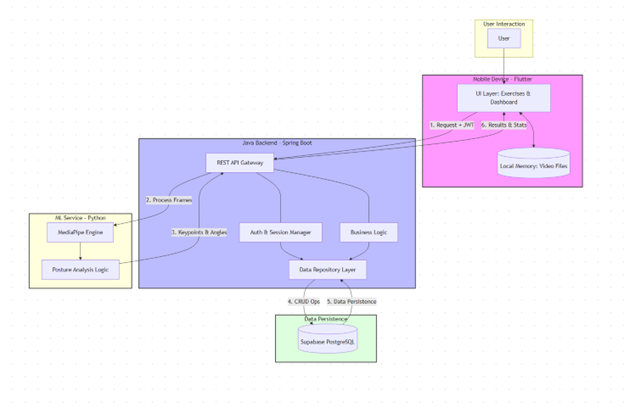
\includegraphics[width=0.85\textwidth]{./figures/system_architecture.png}
    \caption{High-level architecture of the PoseFix system, showing the three-tier structure and the data flow between components.}
    \label{fig:architecture}
\end{figure}

The \textbf{Flutter mobile application} serves as the user interface layer. It communicates exclusively with the Java backend over HTTP and relies on the Supabase client SDK only for authentication token management. The mobile client never contacts the Python ML service directly.

The \textbf{Java Spring Boot backend} is responsible for authentication enforcement, business logic, data persistence, and orchestration. When a user submits a video for analysis, the backend stores the file locally, forwards it to the Python service by reference, receives the result, persists it to the database, and returns it to the mobile client. The backend is also the sole layer that communicates with the Supabase PostgreSQL database.

The \textbf{Python FastAPI ML service} is a stateless microservice with a single responsibility: accepting a file path and an exercise identifier, processing the video using MediaPipe BlazePose, evaluating the pose against rule-based heuristics, and returning a structured JSON result. It holds no database connection and no user state.

\textbf{Supabase} provides two infrastructure services: the authentication layer, where user identity is managed and JWT tokens are issued, and the PostgreSQL database, where all application data is persisted.

This architecture offers several advantages relevant to the thesis context. The ML service can be developed, tested, and restarted independently of the backend. The backend can be extended with new business features without modifying the ML logic. The mobile client requires only knowledge of the backend API contract.

\subsection{Technology Stack}
\label{subsec:tech-stack}

\begin{table}[htbp]
\begin{center}
\begin{tabular}{|p{100pt}|p{200pt}|}
\hline
\textbf{Layer} & \textbf{Technology} \\
\hline
Mobile & Flutter (Dart), Supabase Auth SDK, GoRouter, Provider \\
\hline
Backend & Java 17, Spring Boot 3.x, Spring Security, Spring Data JPA \\
\hline
ML Service & Python 3.11, FastAPI, MediaPipe Tasks API, OpenCV, NumPy \\
\hline
Database & Supabase (PostgreSQL 15), Row Level Security \\
\hline
Authentication & Supabase Auth (JWT) \\
\hline
\end{tabular}
\end{center}
\caption{Technology stack used in the PoseFix system.}
\label{tab:techstack}
\end{table}

\section{User Journey}
\label{sec:user-journey}

Figure \ref{fig:userjourney} presents the complete user journey through the PoseFix application, from initial registration to viewing posture feedback and tracking progress.

\begin{figure}[htbp]
    \centering
    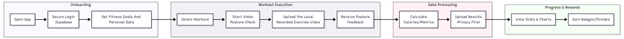
\includegraphics[width=0.90\textwidth]{./figures/user_journey.png}
    \caption{User journey through the PoseFix application, covering onboarding, workout execution, data processing, and progress tracking.}
    \label{fig:userjourney}
\end{figure}

The journey is divided into four phases.

\textbf{Onboarding} covers initial registration via Supabase Auth, followed by the user entering personal data: name, birth date, height, weight, and sex. This data is stored in the \texttt{profiles} table and used for contextualisation of feedback in future versions.

\textbf{Workout Execution} is the core operational loop. The user creates a workout session and adds one or more exercises to it, each with its own sets, reps, and load. For any exercise within the session, the user may record a video of themselves performing that exercise and upload it for analysis. The system returns a posture score, a list of detected mistakes with severity ratings, and a summary of measured joint angles specific to that exercise entry.

\textbf{Data Processing} occurs server-side and is transparent to the user. The backend receives the video, stores it temporarily, invokes the ML service, persists the result linked to the specific workout exercise entry, and deletes the video file. Only the structured analysis metadata is retained in the database.

\textbf{Progress and Tracking} allows the user to review their workout history, track weight trends over time, and compare posture scores across sessions to observe improvement.

\section{Database Design}
\label{sec:database}

The database schema consists of six tables managed by Supabase PostgreSQL. Figure \ref{fig:erd} illustrates the entity-relationship structure.

\begin{figure}[htbp]
    \centering
    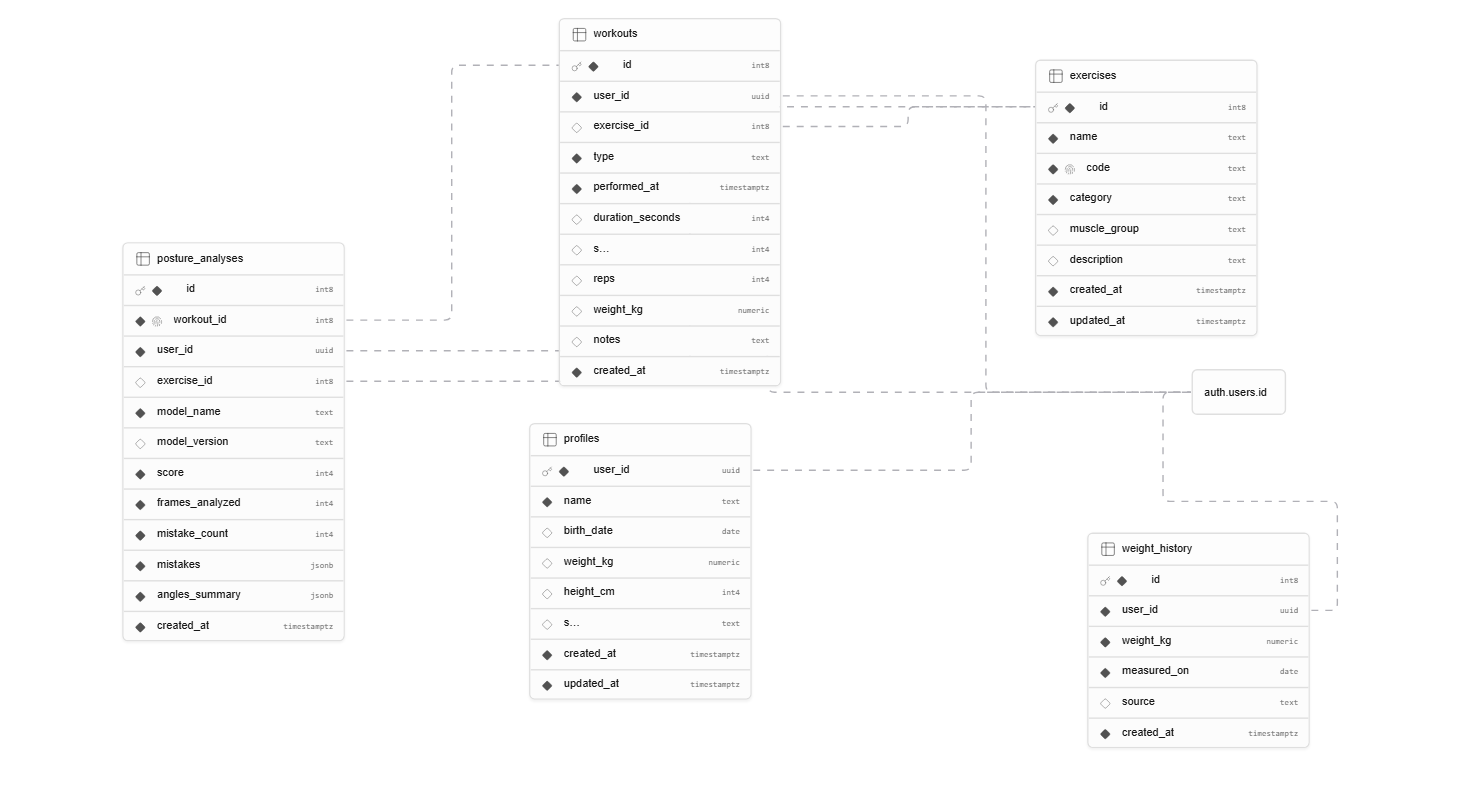
\includegraphics[width=0.85\textwidth]{./figures/erd_diagram.png}
    \caption{Entity-relationship diagram of the PoseFix database schema.}
    \label{fig:erd}
\end{figure}

\textbf{profiles} holds one record per user, linked to the Supabase \texttt{auth.users} table via the \texttt{user\_id} primary key. It stores name, birth date, height, weight, and sex. An update trigger automatically maintains the \texttt{updated\_at} timestamp.

\textbf{weight\_history} records one weight measurement per user per calendar day, enforced by a unique index on \texttt{(user\_id, measured\_on)}. This design prevents multiple daily entries that could distort trend visualisations.

\textbf{exercises} is a static reference table defining the supported exercises by name, code, category, and muscle group. The \texttt{code} column (e.g. \texttt{lat\_pulldown}) is used as a stable identifier for routing within the ML service.

\textbf{workouts} records a training session at the session level. Each row is owned by a user and stores the session timestamp, type, total duration, and optional notes. Crucially, it does not store per-exercise details such as sets, reps, or load — these are delegated to the \texttt{workout\_exercises} table, allowing a single session to contain multiple exercises.

\textbf{workout\_exercises} is a line-item table that links a workout session to a specific exercise and captures the execution parameters: \texttt{sets}, \texttt{reps}, \texttt{weight\_kg}, and \texttt{order\_index}. The \texttt{order\_index} field preserves the sequence in which exercises were performed within the session. This design normalises the schema and removes the one-exercise-per-session constraint that would otherwise limit the application's utility.

\textbf{posture\_analyses} holds the result of a video analysis for a specific exercise within a workout. It is linked one-to-one with a \texttt{workout\_exercises} row via the \texttt{workout\_exercise\_id} foreign key, ensuring that each individual exercise entry can have at most one analysis. The \texttt{mistakes} and \texttt{angles\_summary} columns are stored as JSONB, allowing the flexible structure returned by the ML service to be persisted without a fixed schema. Additional metadata includes the model name and version used for the analysis, the number of frames processed, and the total mistake count.

The relationships between tables follow a clear ownership hierarchy:

\begin{equation}
    \texttt{auth.users} \xrightarrow{1:1} \texttt{profiles} \xrightarrow{1:N} \texttt{workouts} \xrightarrow{1:N} \texttt{workout\_exercises} \xrightarrow{1:1} \texttt{posture\_analyses}
    \label{eq:dbrel}
\end{equation}

The \texttt{exercises} reference table participates in the schema via a foreign key from \texttt{workout\_exercises}, and independently from \texttt{posture\_analyses}, so that the analysed exercise is always traceable regardless of whether the originating workout entry is still present. Weight history is independently owned by the user and does not participate in the workout chain.
